\chapter{Пример результата работы программы}\label{appendix-extra-examples}
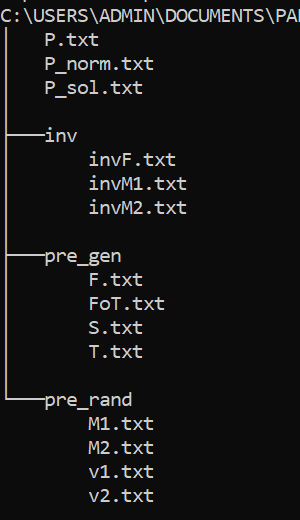
\includegraphics [scale=0.8]{my_folder/images/4}
\captionof{figure}{Пример результата: файловая структура}
\\
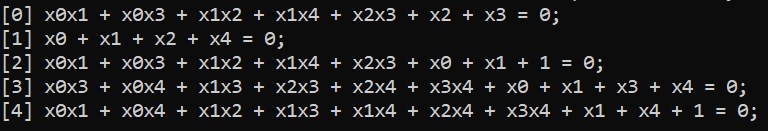
\includegraphics [scale=0.8]{my_folder/images/5}
\captionof{figure}{Пример результата: сгенерированная система уравнений (файл P.txt)}
\\
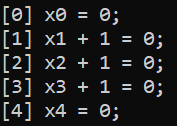
\includegraphics [scale=0.8]{my_folder/images/6}
\captionof{figure}{Пример результата: решение системы уравнений (файл P\_sol.txt)}
\\
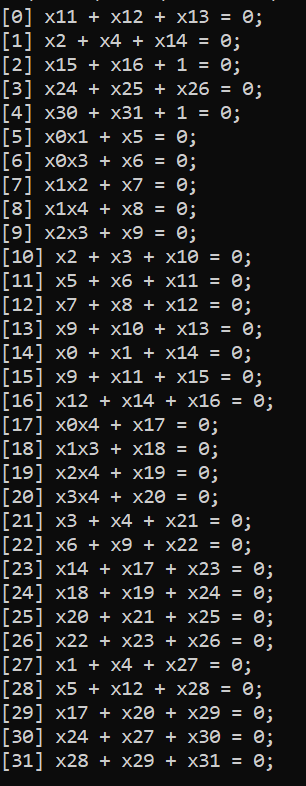
\includegraphics [scale=1]{my_folder/images/7}
\captionof{figure}{Пример результата: нормализованная система уравнений (файл P\_norm.txt)}
\\
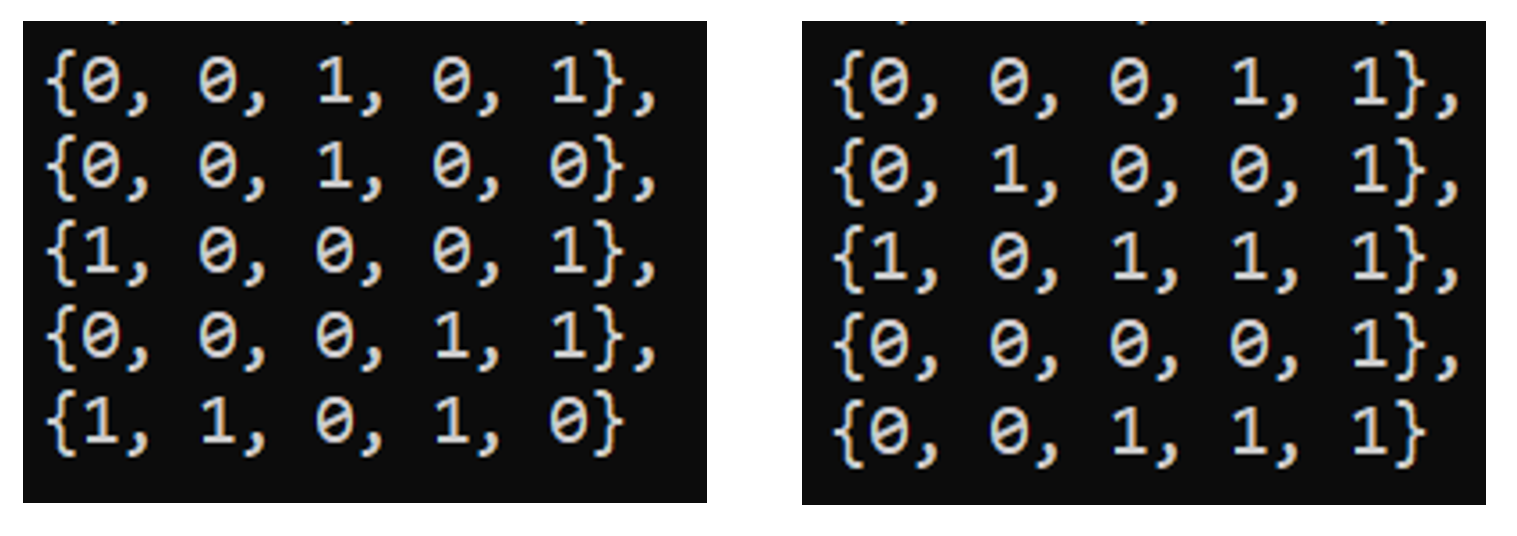
\includegraphics [scale=1]{my_folder/images/8}
\captionof{figure}{Пример результата: случайно сгенерированные матрицы М1 и М2 (файлы M1.txt и M2.txt)}
\\
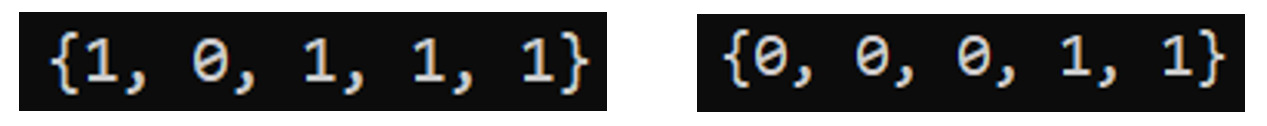
\includegraphics [scale=1]{my_folder/images/9}
\captionof{figure}{Пример результата: случайно сгенерированные векторы v1 и v2 (файлы v1.txt и v2.txt)}
\\
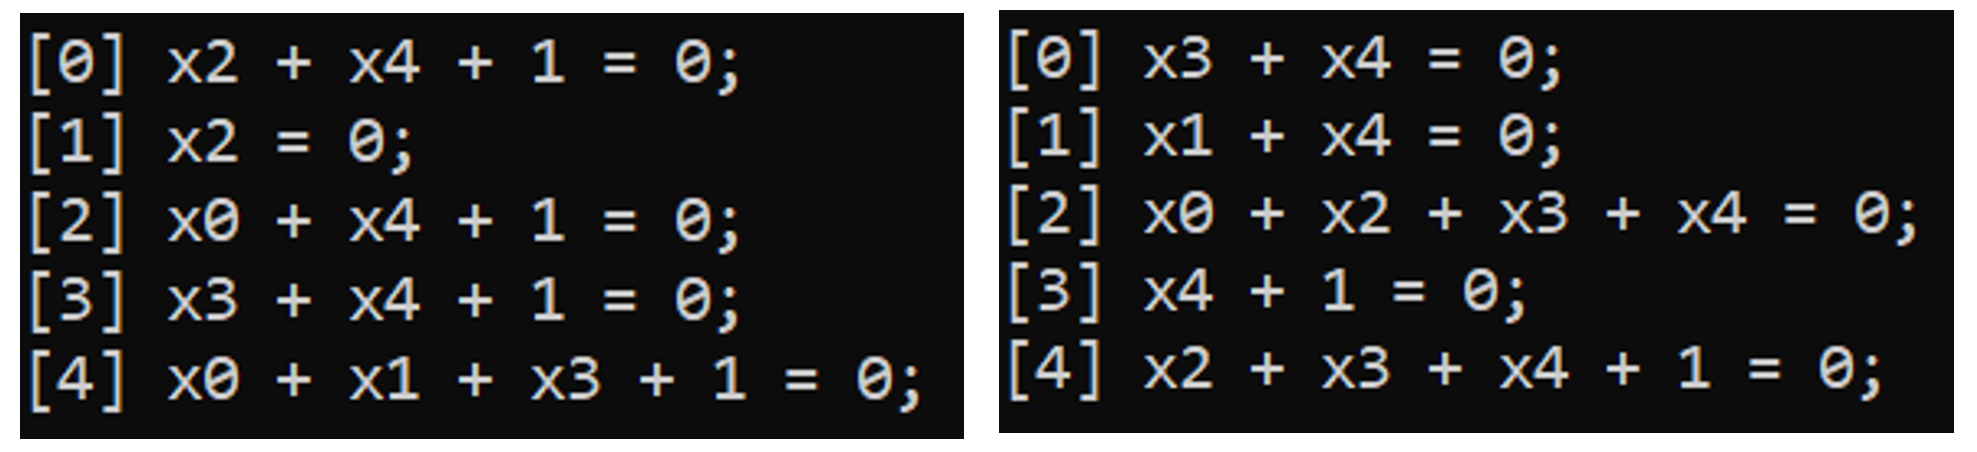
\includegraphics [scale=1]{my_folder/images/10}
\captionof{figure}{Пример результата: преобразования S и T (файлы S.txt и T.txt)}
\\
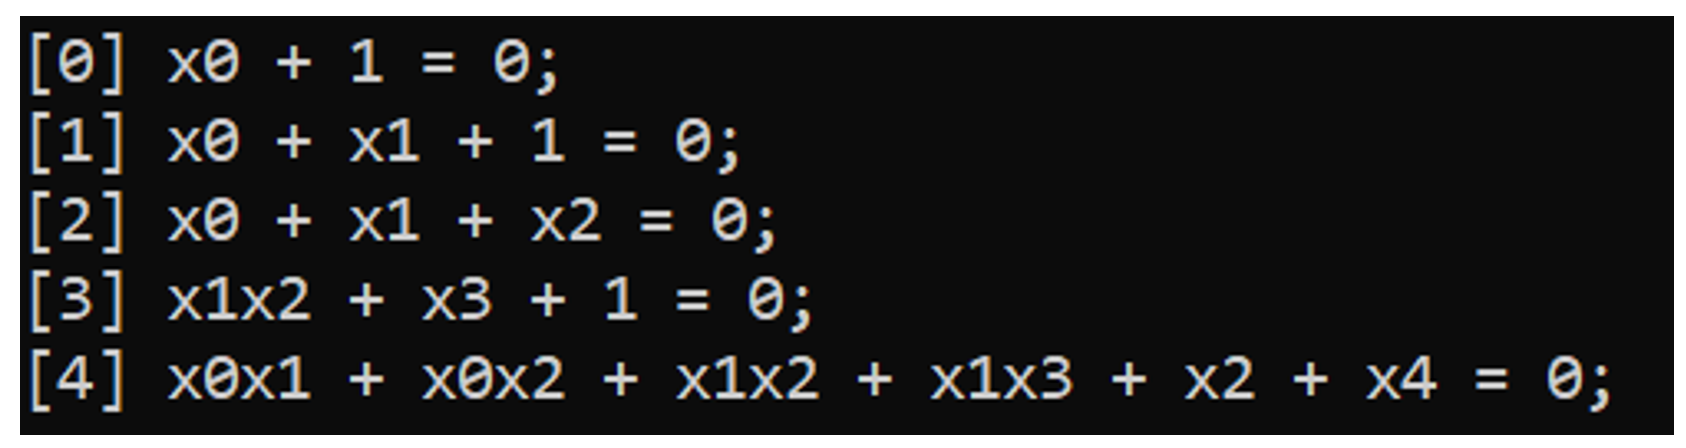
\includegraphics [scale=1]{my_folder/images/11}
\captionof{figure}{Пример результата: преобразование F (файл F.txt)}
\\

\newpage

\chapter{Структура программного решения}\label{appendix-extra-examples}
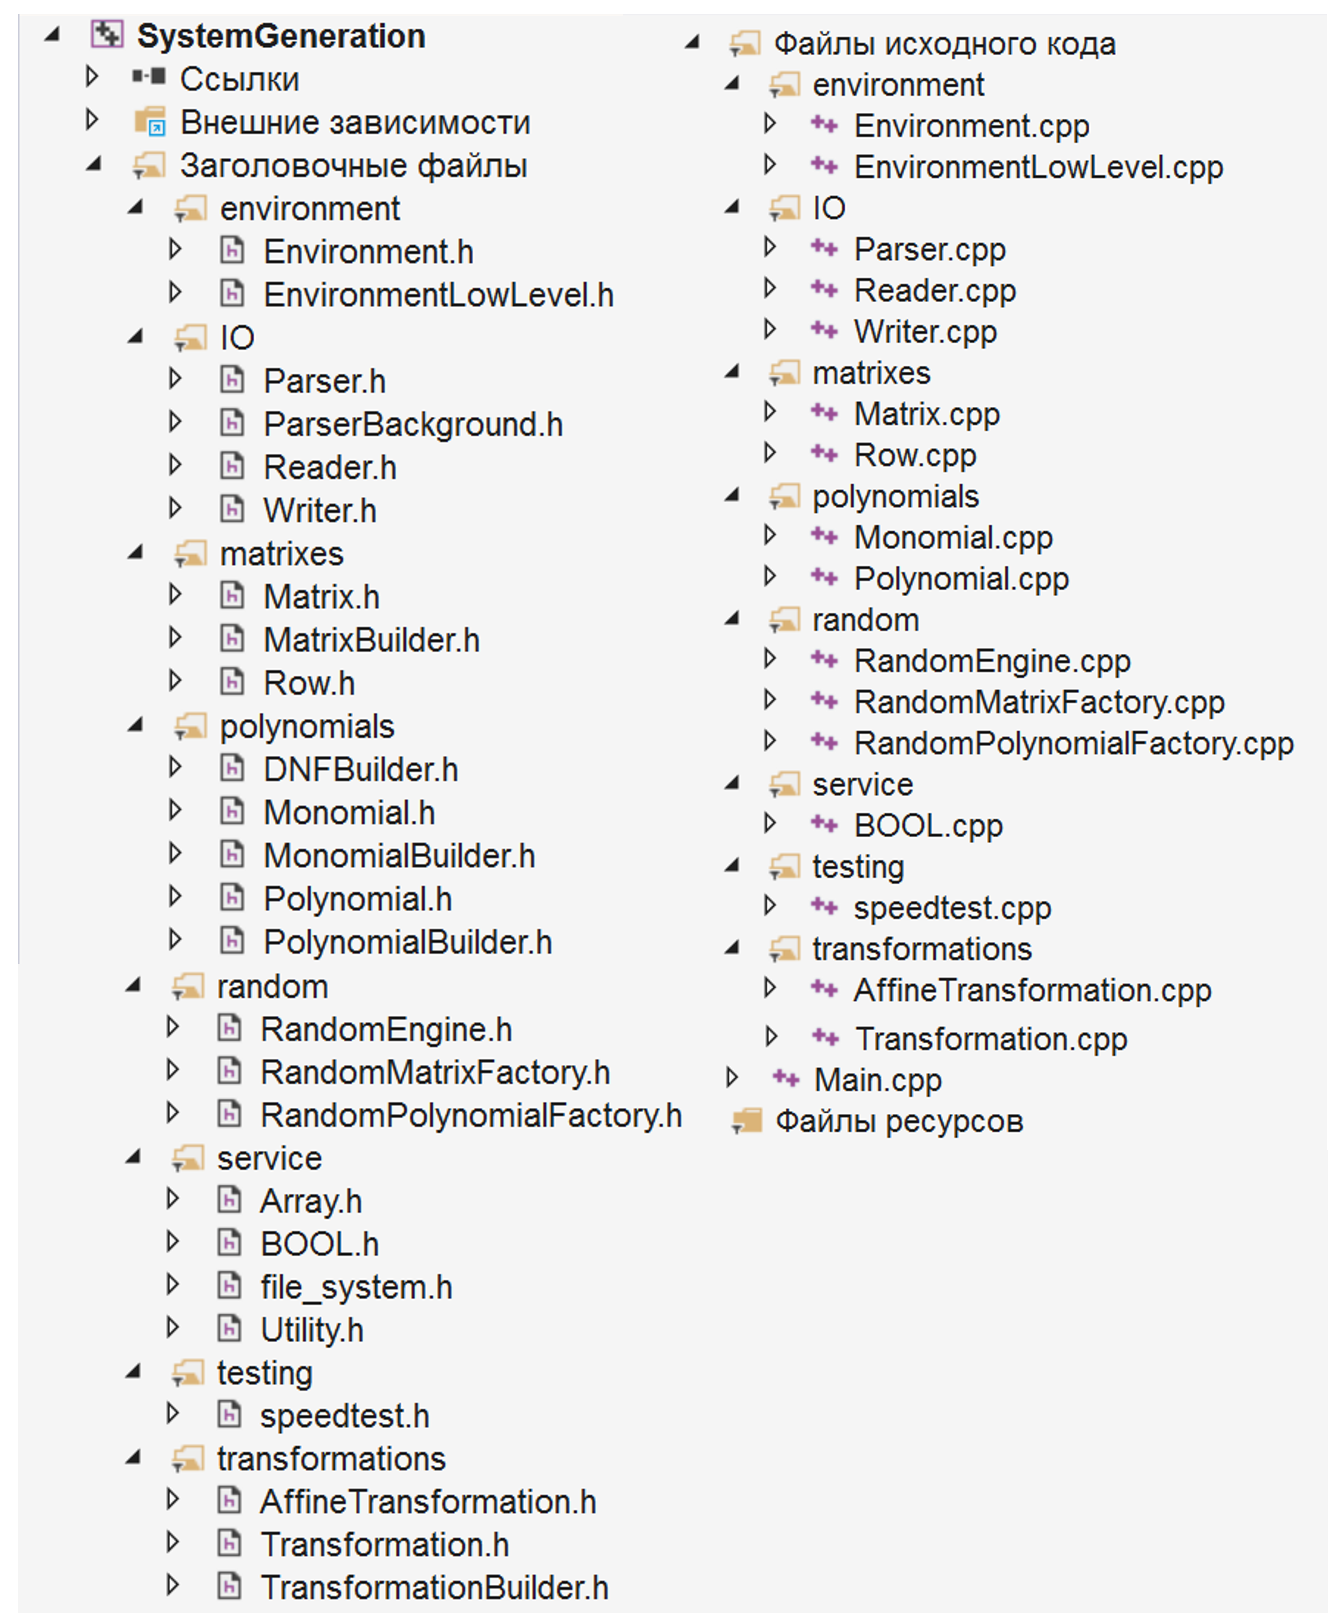
\includegraphics [scale=1.3]{my_folder/images/12}
\captionof{figure}{Представление файлов решения в виде списка}
\\ 

\chapter{Код высокоуровневой реализации алгоритмов}\label{appendix-extra-examples}

\section{Генерация системы уравнений}
void EnvironmentLowLevel::generateSystem(bool print\_or\_not)
\{
\\
	if (print\_or\_not) cout << "Performing preparations... "; \\
	IO::Writer writer(foldername);\\
	std::mt19937 gen = RandomEngine().getRandomEngine();\\
	RandomMatrixFactory<BOOL> matr\_factory(gen);\\
	RandomPolynomialFactory pol\_factory(gen);\\
	\\
	if (print\_or\_not) cout << ''finished'' << endl\\
	<< "Generating random matrixes M1 and M2 and random\\ vectors v1 and v2... ";\\
	\\
	MatrixB m1, m2;\\
	RowB v1(n), v2(n);\\
	matr\_factory.getRandomMatrix(m1, n);\\
	matr\_factory.getRandomMatrix(m2, n);\\
	matr\_factory.getRandomRow(v1);\\
	matr\_factory.getRandomRow(v2);\\
	\\
	MatrixB invM1, invM2; // потребуются позже, при построении решения\\
	invM1.initInverse(m1);\\
	invM2.initInverse(m2);\\
	\\
	if (print\_or\_not) cout << '' finished'' << endl <<\\ "Generating affine transformation S... ";\\
	\\
	AffineTransformation S = AffineTransformation(m1, v1, print\_or\_not);\\
	if (print\_or\_not) cout << '' finished'' << endl << "Generating affine transformation T... ";\\
	AffineTransformation T = AffineTransformation(m2, v2, print\_or\_not);\\
	\\
	if (print\_or\_not) cout << '' finished'' << endl << "Generating random transformation F... ";\\
	\\
	// Строим преобразование F\\
	TransformationBuilder builder;\\
	Polynomial cur;\\
	size\_t prev\_num = 0;\\
	for (int i = 0; i < n; i++)\{\\
		pol\_factory.getQuadraticPolynomial(cur, i);\\
		cur += Monomial(i);\\
		builder << cur;\\
		if (print\_or\_not) \{\\
			if ((i + 1) \% 10 == 0)\{\\
				for (size\_t i2 = 0; i2 < prev\_num; i2++)\\ cout << '\b';\\
				cout << (i + 1) << '/' << n;\\
				prev\_num = to\_string(i + 1).length() + to\_string(n).length() + 1;\\
			\}\\
		\}\\
	\}\\
	if (print\_or\_not)\\
	for (size\_t i = 0; i < prev\_num; i++)\\
	cout << '\b';\\
	prev\_num = 0;\\
	Transformation F;\\
	builder >> F;\\
	if (print\_or\_not) cout << '' finished'' << endl << "Building inverted F... ";\\
	\\
	// Строим преобразование, обратное к F\\
	// ti = gi(x0..x(i-1)) + xi => xi = gi(t0..t(i-1)) + ti\\
	Transformation invF;\\
	vector<Polynomial> trans = vector<Polynomial>(1, F[0]); // текущее состояние обратного преобразования\\
	for (int i = 1; i < n; i++)\{\\
		Polynomial g\_i = F[i]; // зависит от t0..t(i-1)\\
		g\_i += {i};\\
		\\
		Transformation g\_i\_x; // g\_i (x0, x1, ..., x(i-1))\\
		g\_i\_x.initComposition(trans, g\_i);\\
		g\_i = g\_i\_x[0]; // зависит уже от x0..x(i-1)\\
		\\
		g\_i += { i }; // теперь это выражение для x\_i\\
		trans.push\_back(g\_i);\\
		\\
		if (print\_or\_not) \{\\
			for (size\_t i2 = 0; i2 < prev\_num; i2++)\\
			cout << '\b';\\
			cout << (i + 1) << '/' << n;\\
			prev\_num = to\_string(i + 1).length() + to\_string(n).length() + 1;\\
		\}\\
	\}\\
	if (print\_or\_not)\\
	for (size\_t i = 0; i < prev\_num; i++) cout << '\b';\\
	invF = trans;\\
	\\
	if (print\_or\_not) cout << '' finished'' << endl << "Building composition P = SoFoT... ";\\
	\\
	// строим итоговое преобразование P\\
	Transformation FT, P;\\
	FT.initComposition(T, F);\\
	P.initComposition(FT, S);\\
	\\
	if (print\_or\_not) cout << '' finished'' << endl << "Printing into files... ";\\
	\\
	writer.print(v1, "pre\_rand/v1.txt");\\
	writer.print(v2, "pre\_rand/v2.txt");\\
	writer.print(m1, "pre\_rand/M1.txt");\\
	writer.print(m2, "pre\_rand/M2.txt");\\
	writer.print(invM1, "inv/invM1.txt");\\
	writer.print(invM2, "inv/invM2.txt");\\
	writer.print(S, "pre\_gen/S.txt");\\
	writer.print(T, "pre\_gen/T.txt");\\
	writer.print(F, "pre\_gen/F.txt");\\
	writer.print(FT, "pre\_gen/FoT.txt");\\
	writer.print(P, "P.txt");\\
	writer.print(invF, "inv/invF.txt");\\
	\\
	if (print\_or\_not) cout << '' finished'' << endl;\\
\}\\


\section{Решение системы уравнений}
Данная функция используется также для проверки правильности построения обратного преобразования. При решении первый параметром передается вектор, состоящий из нулей, а третьим – логическое значение \(true\). При проверке правильности построения обратного преобразования первым параметром передается случайно сгенериованный вектор, а третьим – логическое значение \(false\), и результат (содержимое ссылки, передаваемой вторым параметром) сравнивается с вектором, переданным первым параметром.\\

void EnvironmentLowLevel::getInvert(const std::vector<BOOL>\& in, std::vector<BOOL>\& out, bool print\_to\_file\_or\_not)\{\\
	\\
	RowB v1(n), v2(n);\\
	MatrixB invM1, invM2;\\
	Transformation invF;\\
	IO::Reader reader(foldername);\\
	IO::Writer writer(foldername);\\
	reader.read(v1, "pre\_rand/v1.txt");\\
	if (v1.size() == 0) throw exception("Cannot read files");\\
	\\
	reader.read(v2, "pre\_rand/v2.txt");\\
	reader.read(invM1, "inv/invM1.txt");\\
	reader.read(invM2, "inv/invM2.txt");\\
	reader.read(invF, "inv/invF.txt");\\
	\\
	RowB invS(n); // invS(c) = invM1*(c + v1)\\
	RowB invFS(n); // invF(invS(c))\\
	RowB invTFS(n);  // invP = invT(invF(invS(c))) = invM2*(invF(invS(c)) + v2)\\
	\\
	v1.xor(in);\\
	invM1.multiply(v1, invS); \\
	\\
	vector<BOOL> invS2, res;\\
	invS.toVector(invS2);\\
	invF.substitute(invS2, res);\\
	invFS = res;\\
	\\
	invFS.xor(v2);\\
	invM2.multiply(invFS, invTFS);\\
	\\
	if (print\_to\_file\_or\_not)\{\\
		TransformationBuilder builder;\\
		for (int i = 0; i < n; i++)\{\\
			if (invTFS.get(i) == TRUE)\\
			builder << vector<Monomial> \{ i, FREE\_MEMBER \};\\
			else 
			builder << vector<Monomial> \{ i \};\\
		\}\\
		Transformation solution;\\
		builder >> solution;\\
		\\
		writer.print(solution, "P\_sol.txt");\\
	\}\\
	\\
	invTFS.toVector(out);\\
\}\\


\section{Нормализация системы уравнений}

void transformations::Transformation::normalize() \{\\
	int n\_core = (int)coordinates.size();\\
	\\
	// z - номер переменнной к добавлению\\
	int z = 0;\\
	for (int i = 0; i < n\_core; i++) \{\\
		if (coordinates[i].get\_n\_max() > z)
		z = coordinates[i].get\_n\_max();\\
	\}\\
	z++;\\
	\\
	for (int i = 0; i < n\_core; i++) \{\\
		Polynomial Lr;\\
		auto beg = coordinates[i].begin();\\
		auto mark = beg; // указывает на последний добавленный моном (сразу же добавим)\\
		\\
		while
		(mark < coordinates[i].begin() + coordinates[i].size() - 1
		\&\& !(mark == coordinates[i].begin() + coordinates[i].size() - 2 \&\& *(mark + 1) == FREE\_MEMBER)
		\&\& !coordinates[i].is\_standard()) {\\
			Lr += *mark;\\
			Lr += Monomial(z);\\
			\\
			if (Lr.is\_standard()) \{\\
				coordinates.push\_back(Lr);\\
				Lr += Monomial(z);\\
				int sz = (int)coordinates.size() - 1; // без последнего\\
				for (int j = 0; j < sz; j++)\\
				coordinates[j].replace(Lr, z);\\
				z++;\\
				\\
				mark = coordinates[i].begin();\\
				Lr.clear();\\
			\} else \{\\
				Lr += Monomial(z);\\
				mark++;\\
			\}
		\}
	\}
\}
